\documentclass[letterpaper,journal]{IEEEtran}
\usepackage{amsmath,amssymb,amsfonts}
\usepackage{algorithmic}
\usepackage{algorithm}
\usepackage{graphicx}
\usepackage{booktabs}
\usepackage{xcolor}
\usepackage[colorlinks=true,allcolors=blue]{hyperref}
\usepackage{url}

\newcommand{\Lie}{\dot{V}}
\newcommand{\xstar}{x^\star}
\newcommand{\Vstar}{V^\star}

\begin{document}

\title{Formal Certification of Neural Lyapunov Functions\\ for Transient Stability in Lossy Power Networks}

\author{Sehaj Singh%
\thanks{Problem formulation and supervision by Prof. Wenqi Cui, NYU Tandon ECE.
This work is simulation only.}}

\markboth{Working paper, 2026}{Singh: Certified Neural Lyapunov Functions for Transient Stability}
\maketitle

\begin{abstract}
A neural Lyapunov function trained against randomly sampled violations cannot be
certified, because a certificate quantifies over every point in a region while
sampling only ever visits a measure-zero subset, so a network can report a
$99.98\%$ empirical satisfaction rate and still fail the Lyapunov conditions on a
set that random sampling never lands on. We reproduce the Lyapunov-regularized
reinforcement learning of Cui and Zhang for the lossy Kron-reduced New England
39-bus swing model, then show with the neural network verifier CROWN that the
as-trained value function violates both the positive-definiteness condition and
the Lie-derivative condition through genuine counterexamples that a directed
search finds immediately while $200{,}000$ random samples find none. We then close
the loop, using the verifier itself as the sampler and feeding its
counterexamples back into training, so the same architecture that certifies over
nothing becomes certifiable over a real region: on the projected gen-5 slice that
matches the authors' own figure, counterexample-guided training certifies the
Lie-derivative condition out to a sublevel radius $\rho=1.5$ and an exponential
decrease rate $\beta$ up to $3.97$, both audited by an independent attack. The
certified region collapses as the state dimension grows, which is quantified
rather than hidden and which points directly at where the next work has to go.
\end{abstract}

\begin{IEEEkeywords}
Neural Lyapunov functions, transient stability, formal verification, CROWN,
branch-and-bound, counterexample-guided training.
\end{IEEEkeywords}

\section{Introduction}
Transient stability of a power network asks whether the generators, after a
disturbance, swing back to a synchronous equilibrium rather than losing
synchronism. The classical certificate is an energy function, but for a network
with resistive losses the conductance coupling enters the swing equations as a
term $G_{ij}\cos(\delta_i-\delta_j)$ that is not the gradient of any scalar, so
no analytic energy function exists~\cite{chiang1989energy}. That single term is
why a valid Lyapunov function for lossy frequency dynamics has been an open
problem for decades, and it is the entire reason the frequency-control problem is
interesting while the voltage-control problem, whose dynamics are linear, is not.

Cui and Zhang sidestep the non-existence result by \emph{learning} a Lyapunov
function $V_\phi$ as a neural network, jointly with a decentralized controller,
under a training loss that penalizes violations of the Lyapunov conditions on
sampled states~\cite{cui2022lyapunov}. Their method works well empirically, and
the last sentence of their paper names the gap it leaves open: an important
direction is to verify whether the learned function satisfies the Lyapunov
conditions for \emph{all} points in a region, not just on samples. They report the
Lie derivative is slightly positive on about $0.1\%$ of sampled points after
training. Sampling is not a proof, because the conditions are universally
quantified over a continuous region while any sample set is finite, so the
question their paper poses is exactly the question a verifier answers.

This paper answers it. We reproduce their training, we use the neural network
verifier CROWN~\cite{zhang2018crown} with branch-and-bound over the nonlinear
swing dynamics to certify the Lyapunov conditions over a region rather than a
sample, and where the as-trained network fails we close the loop with
counterexample-guided training. The contribution is not a single verified box, it
is the demonstration that the sampling-to-certification gap is real and directed,
that it is the same gap in the condition that was supposed to be trivial, and that
feeding a sound verifier's counterexamples back into training is what converts an
uncertifiable network into a certifiable one over a real region.

\section{Related Work}
Certifying a learned Lyapunov function means proving a nonlinear inequality over a
continuous region, and the tools differ in what nonlinearities they admit and how
they scale. Satisfiability-modulo-theories methods with a $\delta$-complete
solver certify neural Lyapunov controllers exactly~\cite{chang2019neural}, which
is the approach Cui and Zhang cite, but they scale poorly and are typically
tractable only for small systems, which is why their own paper notes the
limitation. Mixed-integer encodings require piecewise-linear activations and so
cannot represent the ELU network used here at all. Sum-of-squares programming
requires polynomial dynamics and so cannot represent the $\sin$ and $\cos$ of the
swing equations. Learned-dynamics constructions that build stability in by
design~\cite{manek2019stable} avoid verification but change the model class.

Bound propagation with branch-and-bound occupies a different point. CROWN
propagates a sound linear relaxation of a general nonlinear computation
graph~\cite{zhang2018crown}, its automatic-differentiation implementation
auto\_LiRPA bounds arbitrary graphs~\cite{xu2020autolirpa}, $\beta$-CROWN adds
per-neuron branching for completeness~\cite{wang2021betacrown}, and GenBaB
extends branch-and-bound to general nonlinearities including $\sin$, $\cos$, and
the ELU derivative~\cite{shi2024genbab}. The bounds are GPU-parallel across
subdomains and, being differentiable, can be trained
against~\cite{shi2024certified}. This is the reason CROWN, and not SMT, is the
right tool for a lossy swing model with an ELU value function: it handles the
exact operators the problem contains, and it hands back a counterexample when it
fails rather than only a verdict. Our formulation of the Lie derivative as a
boundable graph and the sublevel-set region-of-attraction follow the neural
control verification line~\cite{yang2024lyapunov} and its
tutorial~\cite{tutorial2026abcrown}.

\section{Problem Formulation}
\subsection{Lossy swing dynamics}
The New England 39-bus system is Kron-reduced to its $n=10$ generator buses. With
state $x=(\delta,\omega)\in\mathbb{R}^{2n}$ the swing dynamics
are~\cite{cui2022lyapunov}
\begin{align}
\dot{\delta}_i &= \omega_i, \\
M_i\dot{\omega}_i &= P_i - D_i\omega_i - u_i(\omega_i)
 - \sum_{j} B_{ij}\sin(\delta_i-\delta_j)
 - \sum_{j} G_{ij}\cos(\delta_i-\delta_j),
\end{align}
where $B_{ij}$ is the susceptance coupling and $G_{ij}$ is the conductance
coupling produced by network losses. We match the authors' training dynamics,
which integrate $\dot\delta_i = \omega_{\mathrm{scale}}\,\omega_i$ with
$\omega_{\mathrm{scale}}=2\pi$ because their $\omega$ is a per-unit frequency in
Hz, and which fold the damping $D_i\omega_i$ into the controller, so the certified
closed loop is $f(x,u(x))$ with $u$ supplying the damping.

\subsection{Controller and Lyapunov network}
The certified controller is the saturated linear droop law
$u_i(\omega_i)=\mathrm{sat}(c_i\omega_i)$ that the authors use while training
$V_\phi$; it is piecewise linear, so CROWN handles it exactly. The value function
$V_\phi(\delta,\omega)$ is a single-hidden-layer network with ELU activations,
chosen for a smooth bounded derivative, evaluated on the reference-subtracted
coordinates $z=[\delta_i-\delta_1,\ \omega_i-\omega_1]$ of dimension $2(n-1)=18$,
which removes the rotational symmetry of the swing model so the equilibrium is an
isolated point.

\subsection{Lyapunov conditions}
With equilibrium $\xstar$ and $\Vstar=V(\xstar)$, the conditions
are~\cite{cui2022lyapunov}
\begin{align}
\text{(4a)}\quad & V(x) > \Vstar && \text{for } x\neq\xstar, \\
\text{(4b)}\quad & \Lie(x) = \nabla V(x)\cdot f(x,u(x)) < 0 && \text{for } x\neq\xstar, \\
\text{(4c)}\quad & \Lie(\xstar) = 0,
\end{align}
and Proposition 2 strengthens (4b) to an exponential rate,
$\Lie(x) \le -\beta\,(V(x)-\Vstar)$. She named (4a) for certification. We certify
it because she asked, but (4a) is a property of $V$ alone and never touches the
dynamics, so the condition that actually needs the nonlinear swing equations is
(4b) and its Proposition-2 form, and that is where the contribution is.

\section{Verification Formulation}
\subsection{The Lie derivative as a boundable graph}
Condition (4b) requires bounding $\Lie(x)=\nabla V(x)\cdot f(x,u(x))$ over a box,
which means the gradient of $V$ has to be part of the graph the verifier bounds.
For the single-hidden-layer ELU network the gradient is analytic,
\begin{equation}
\nabla_z V = \big(W_2 \odot \mathrm{ELU}'(W_1 z + b_1)\big) W_1,
\quad \mathrm{ELU}'(a)=e^{-\mathrm{relu}(-a)},
\end{equation}
and every operation in it, together with the $\sin$ and $\cos$ of $f$, is a
natively boundable operator, so we express the whole scalar
$F(x)=-\Lie(x)$ as one computation graph and bound it with CROWN directly. This
specializes the general-purpose route, in which auto\_LiRPA's Jacobian operator
expands gradient nodes and GenBaB branches the $\sin$, $\cos$, and ELU
nonlinearities~\cite{shi2024genbab,tutorial2026abcrown}; for a one-hidden-layer
network the analytic gradient graph is exact and its bounds are tighter, so we use
it and keep the Jacobian route available for deeper networks. We also replace the
ELU by the identity $\mathrm{ELU}(x)=\mathrm{relu}(x)-\mathrm{relu}(1-e^{-\mathrm{relu}(-x)})$,
which matches \texttt{torch.nn.ELU} to $6\times 10^{-8}$ and is boundable, since
this build of auto\_LiRPA has no native ELU bound.

\subsection{Certification and the equilibrium}
We certify $F(x)\ge -\epsilon$ over a box $B$ by propagating a sound CROWN lower
bound and branching $B$ on its widest dimension where the bound is inconclusive; a
nonnegative bound on every leaf verifies the box, and a leaf that cannot be split
hands back either a genuine counterexample with $F<-\epsilon$ (the property is
false) or an unresolved region (the bound stayed loose). These two outcomes are
never conflated. Every verified box is then re-checked by an independent
multi-start projected-gradient attack, and a certificate is rejected if the attack
finds any $F<-\epsilon$, which guards against an unsound bound.

The Lie derivative is zero at the equilibrium by construction, so $F=-\Lie$ is
zero there and no region containing $\xstar$ certifies (4b) as a strict
inequality. We handle this the standard way, certifying on an annulus that
excludes a small ball around $\xstar$, and reporting an explicit tolerance
$\epsilon$ with units where one is used. The region-of-attraction result is a
certified sublevel set: we bisect on $\rho$ for the largest
$\{x: V(x)\le\rho\}\cap B$ that verifies, which is forward invariant and is a
certified inner approximation of the region of attraction.

\section{Counterexample-Guided Certification}
The as-trained network fails, so we close the loop. Her own Algorithm 1 already
collects violating samples by random search, so she has half of this idea; the
missing half is that a random sampler visits measure zero while a verifier's
counterexamples are sound and concentrate exactly where the property is violated.

\begin{algorithm}[t]
\caption{Counterexample-guided certification (CEGIS)}
\label{alg:cegis}
\begin{algorithmic}[1]
\STATE \textbf{input:} trained $V_\phi$, target region $B$, controller $u$
\FOR{iteration $k=1,2,\dots$}
  \STATE $\rho_k \leftarrow$ largest certifiable sublevel radius on $B$ (bisection, CROWN + branch-and-bound)
  \STATE $C \leftarrow$ PGD counterexamples maximizing $\Lie$ on the frontier just past $\rho_k$
  \IF{$C=\varnothing$} \STATE \textbf{return} certified $\rho_k$ \ENDIF
  \STATE retrain $V_\phi$ to drive $\Lie<0$ on $C$ and a grid over $B$, keeping $V>\Vstar$ and $\Lie(\xstar)=0$
\ENDFOR
\end{algorithmic}
\end{algorithm}

\section{Case Study: New England 39-bus}
All numbers below trace to a per-seed JSON that a script wrote, and every figure
regenerates from those JSON files.

\subsection{Reproduction and the sampling gap}
The PyTorch port matches the authors' dynamics to $6.4\times 10^{-7}$ against an
independent transcription of their transfer-matrix algebra. Reproducing their
Algorithm 1 gives $99.98\%$ of sampled states with $\Lie\le 0$ and $100\%$ with
$V>\Vstar$, in line with their reported $\approx 99.9\%$. On this same network,
uniform random sampling finds a (4b) violation in $0$ of $200{,}000$ states, while
a directed projected-gradient attack in the same region drives $6.1\%$ of its
starts to a violation, with a maximum Lie derivative of $+199.9$ against
$-9.6$ for the best random sample. The violations are real and the random sampler
never lands on them, which is the empirical case for a verifier
(Fig.~\ref{fig:gap}).

\begin{figure}[t]
\centering
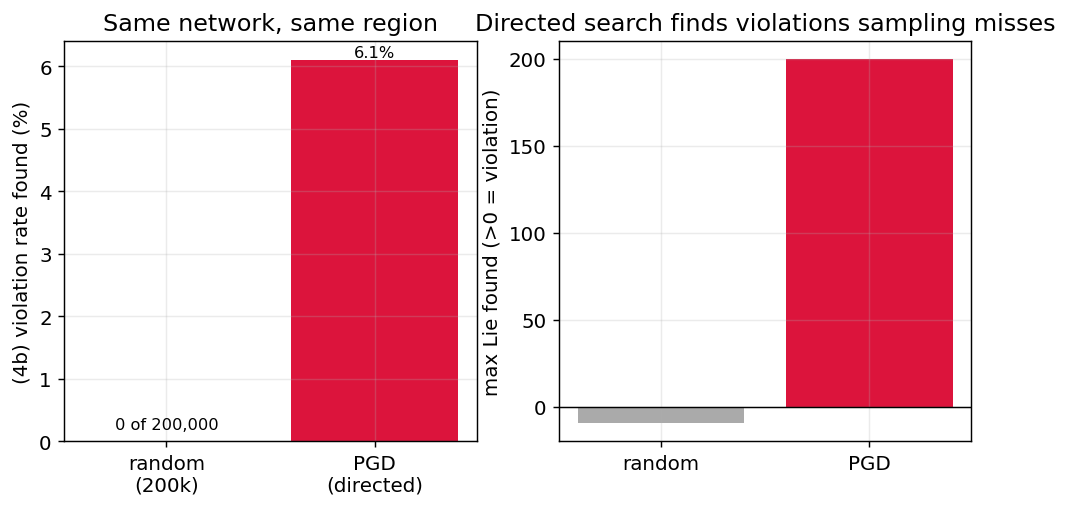
\includegraphics[width=\columnwidth]{figures/sampling_gap.png}
\caption{Same network, same region. Random sampling finds no (4b) violation in
$200{,}000$ draws, a directed attack finds them at $6.1\%$. Sampling statistics
do not certify.}
\label{fig:gap}
\end{figure}

\subsection{The certification staircase}
Branch-and-bound cost grows with input dimension, so we report a staircase rather
than claim full-state verification (Table~\ref{tab:staircase}). On the two-machine
gate, a 4-D lossy system, the pipeline certifies (4b) on a real annulus, which is
the correctness check. On the gen-5 projected slice, the 2-D geometry of the
authors' own Fig.~2, the as-trained network has a genuine (4b) counterexample with
$\Lie=+5.22$ on the far region, and CROWN's optimized bound is $2.36$ times tighter
than interval propagation on the reference box ($-54.8$ versus $-129.5$). In the
full 20-D state the slice-hardened network genuinely violates (4b) even in a box of
radius $0.01$, because the counterexample-guided training was scoped to the slice
and does not transfer, so the certified full-state radius is reported honestly as
the point where a real counterexample appears, not as a verifier timeout.

\begin{table}[t]
\caption{Certification staircase, condition (4b), seed 0. Certified region is the
sublevel radius $\rho$ (slice) or box radius $r$ (full state). Failures are labeled
genuine (a counterexample exists) or incompleteness (bound too loose).}
\label{tab:staircase}
\centering
\begin{tabular}{@{}llll@{}}
\toprule
Rung & dim & network & result \\
\midrule
1: two-bus     & 4  & trained here & certified $\rho=1.2$, audit $+0.34$ \\
2: gen-5 slice & 2  & as-trained   & genuine viol., $\Lie=+5.22$ \\
2: gen-5 slice & 2  & CEGIS        & certified $\rho=1.5$, audit $+2.43$ \\
3: full state  & 20 & CEGIS        & genuine viol. at $r=0.01$ \\
4: full state  & 20 & CEGIS        & genuine viol. at $r=0.5$, $\Lie=+118$ \\
\bottomrule
\end{tabular}
\end{table}

\subsection{Closing the loop}
On the gen-5 slice, counterexample-guided training turns the uncertifiable
as-trained network into a certified one. The certifiable sublevel radius goes from
$0.0$ to $1.5$, the full grid maximum, after a single CEGIS iteration, the
independent attack then finds a minimum $F$ of $+2.43$ over the certified region,
and no further counterexamples appear through five more iterations
(Fig.~\ref{fig:cegis}). Proposition 2 certifies an exponential decrease rate
$\beta$ up to $3.97$ on the same region, so the result is not a binary
verified-or-not but a certified rate. Pushing the region outward, the certified
sublevel radius reaches $\rho=2.0$ before a genuine counterexample appears at
$\rho=2.5$, and across every rung of the staircase every failure the verifier
reports is a genuine violation with a counterexample rather than an unresolved
loose bound, which says the bounds are tight enough here that not-certified means
false, not merely unproven. The same training also fixes (4a): the
as-trained network has a genuine positive-definiteness counterexample with $V<\Vstar$
on the annulus, which $200{,}000$ training samples reported satisfied on
$100\%$ of draws, and the CEGIS network certifies (4a) there with a dense margin of
$+0.097$ (Fig.~\ref{fig:money}).

\begin{figure}[t]
\centering
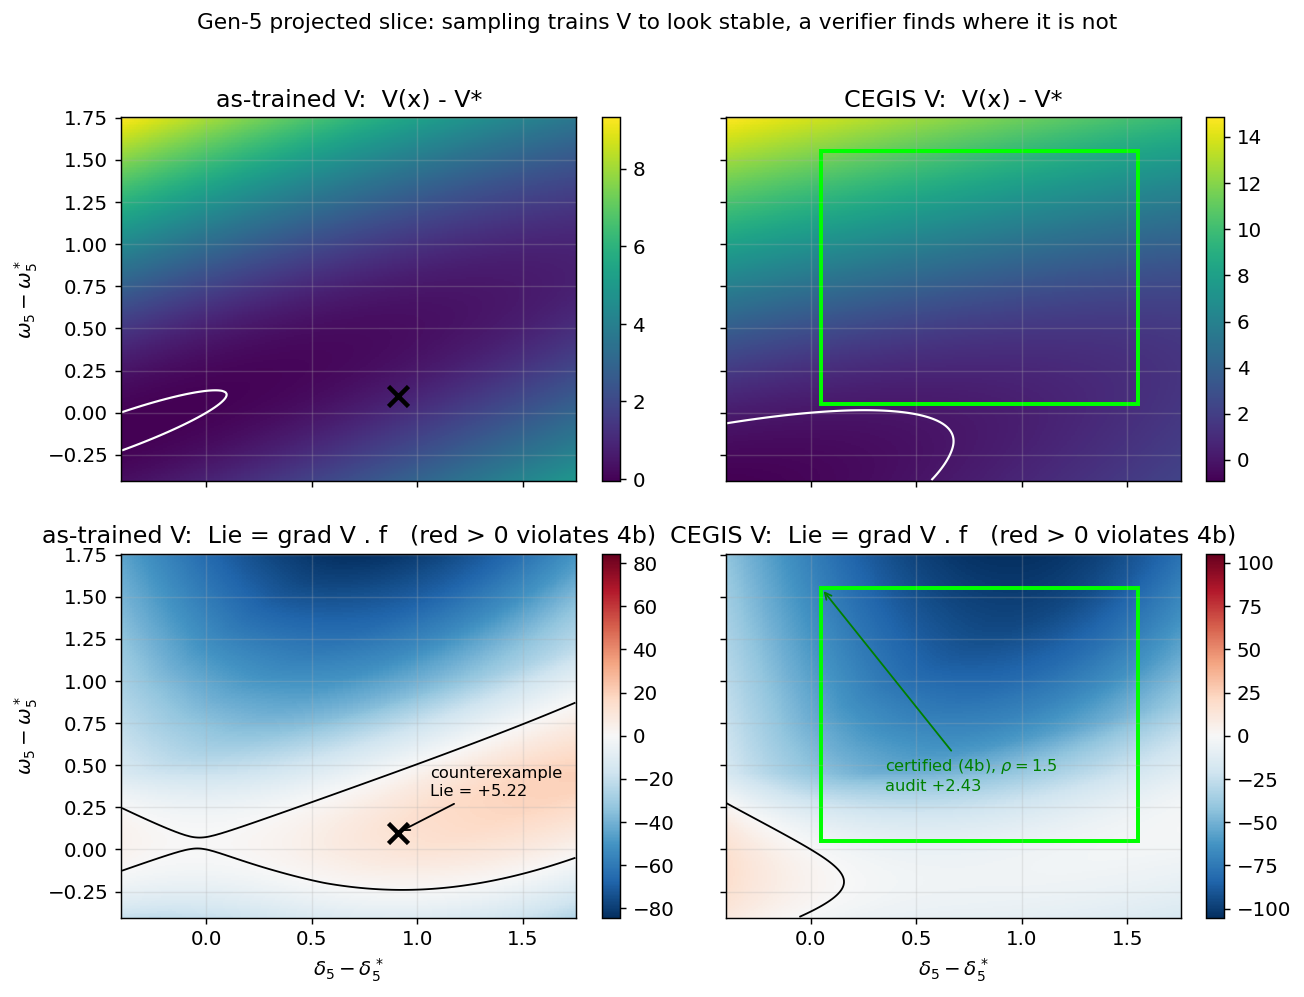
\includegraphics[width=\columnwidth]{figures/money_slice.png}
\caption{Gen-5 projected slice. Top, $V-\Vstar$; bottom, the Lie derivative, red
where positive and so violating (4b). Left, the as-trained network with the
verifier's counterexample marked; right, the CEGIS network with the certified
region drawn in green.}
\label{fig:money}
\end{figure}

\begin{figure}[t]
\centering
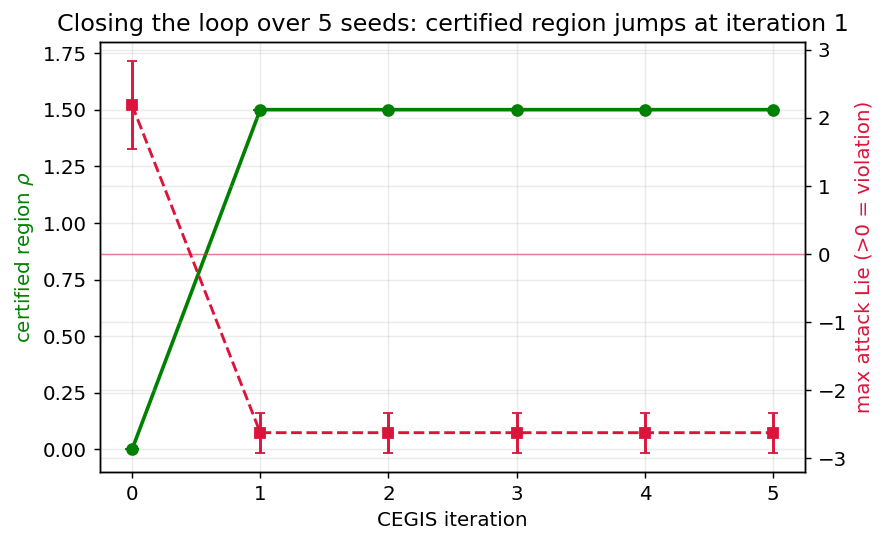
\includegraphics[width=0.92\columnwidth]{figures/cegis_curve.png}
\caption{Certified region against CEGIS iteration. Feeding sound counterexamples
back into training moves the certified sublevel radius from $0$ to $1.5$ in one
step, and the maximum attack Lie derivative drops below zero and stays there.}
\label{fig:cegis}
\end{figure}

\section{Limitations}
The certificate holds over the stated region and nowhere else. The model is the
Kron-reduced lossy swing model that the authors train against, not full AC power
flow, and it omits the explicit damping term, which the controller supplies. The
equilibrium is fixed during training and verification, so a certificate that is
used to assert stability rather than to regularize would have to account for how
the equilibrium moves under load or parameter change, and this one does not.
Verification cost grows with state dimension, and the counterexample-guided
training here was scoped to the projected slice, so the full 20-D result is a
genuine violation rather than a certified region, which is the honest boundary of
the method as it stands. Everything is simulation, with no hardware.

\section{Conclusion}
A learned Lyapunov function that satisfies its conditions on $99.98\%$ of samples
can still be falsified by a verifier that quantifies over the whole region, and
the same verifier's counterexamples, fed back into training, are what certify a
real region on the frequency dynamics that have resisted analytic energy functions
for decades. A certified region that grows under counterexample-guided training is
the first step toward learned grid controllers that ship with a proof rather than a
sampling statistic, and the open problem is that the certified region shrinks as
the state dimension grows, which is where the next work, certified training over
the full state, has to go.

\section*{Acknowledgment}
The author thanks Prof. Wenqi Cui for the problem formulation and supervision, and
for the New England 39-bus lossy-network data, Kron-reduced with the pg-sync-models
toolbox from data in Chow's power system toolbox~\cite{chow1992toolbox}, with droop
coefficients obtained by \texttt{fmincon}.

\bibliographystyle{IEEEtran}
\bibliography{refs}

\end{document}
